% Created 2017-01-20 ven. 08:29
\documentclass[11pt]{article}
\usepackage[utf8]{inputenc}
\usepackage[T1]{fontenc}
\usepackage{fixltx2e}
\usepackage{graphicx}
\usepackage{grffile}
\usepackage{longtable}
\usepackage{wrapfig}
\usepackage{rotating}
\usepackage[normalem]{ulem}
\usepackage{amsmath}
\usepackage{textcomp}
\usepackage{amssymb}
\usepackage{capt-of}
\usepackage{hyperref}
\author{Maxime Chevalier}
\date{\today}
\title{Laboratory Notebook for a Multi-Threaded Version of Quicksort}
\hypersetup{
 pdfauthor={Maxime Chevalier},
 pdftitle={Laboratory Notebook for a Multi-Threaded Version of Quicksort},
 pdfkeywords={},
 pdfsubject={},
 pdfcreator={Emacs 24.5.1 (Org mode 8.3.3)}, 
 pdflang={Frenchb}}
\begin{document}

\maketitle
\tableofcontents


\section{Indroduction}
\label{sec:orgheadline1}
Ce journal est le compte rendu d'un élève de RICM4 à Grenoble.
\section{Caractéristiques de la machine}
\label{sec:orgheadline5}
\subsection{Version du système d'exploitation}
\label{sec:orgheadline2}
\begin{verbatim}
uname -a;
\end{verbatim}

\begin{verbatim}
Linux chevamax-Satellite-Pro-R50-B 4.4.0-21-generic #37-Ubuntu SMP Mon Apr 18 18:33:37 UTC 2016 x86_64 x86_64 x86_64 GNU/Linux
\end{verbatim}

\subsection{CPU}
\label{sec:orgheadline3}
\begin{verbatim}
lscpu;
\end{verbatim}

\begin{center}
\begin{tabular}{lllllllllllllllllllllllllllllllllllllllllllllllllllllllllllllllllllllllllllllllllllllllllll}
Architecture: & x86\(_{\text{64}}\) &  &  &  &  &  &  &  &  &  &  &  &  &  &  &  &  &  &  &  &  &  &  &  &  &  &  &  &  &  &  &  &  &  &  &  &  &  &  &  &  &  &  &  &  &  &  &  &  &  &  &  &  &  &  &  &  &  &  &  &  &  &  &  &  &  &  &  &  &  &  &  &  &  &  &  &  &  &  &  &  &  &  &  &  &  &  &  &  & \\
Mode(s) & opératoire(s) & des & processeurs :32-bit, & 64-bit &  &  &  &  &  &  &  &  &  &  &  &  &  &  &  &  &  &  &  &  &  &  &  &  &  &  &  &  &  &  &  &  &  &  &  &  &  &  &  &  &  &  &  &  &  &  &  &  &  &  &  &  &  &  &  &  &  &  &  &  &  &  &  &  &  &  &  &  &  &  &  &  &  &  &  &  &  &  &  &  &  &  &  &  &  & \\
Byte & Order: & Little & Endian &  &  &  &  &  &  &  &  &  &  &  &  &  &  &  &  &  &  &  &  &  &  &  &  &  &  &  &  &  &  &  &  &  &  &  &  &  &  &  &  &  &  &  &  &  &  &  &  &  &  &  &  &  &  &  &  &  &  &  &  &  &  &  &  &  &  &  &  &  &  &  &  &  &  &  &  &  &  &  &  &  &  &  &  &  &  & \\
CPU(s): & 4 &  &  &  &  &  &  &  &  &  &  &  &  &  &  &  &  &  &  &  &  &  &  &  &  &  &  &  &  &  &  &  &  &  &  &  &  &  &  &  &  &  &  &  &  &  &  &  &  &  &  &  &  &  &  &  &  &  &  &  &  &  &  &  &  &  &  &  &  &  &  &  &  &  &  &  &  &  &  &  &  &  &  &  &  &  &  &  &  & \\
On-line & CPU(s) & list: & 0-3 &  &  &  &  &  &  &  &  &  &  &  &  &  &  &  &  &  &  &  &  &  &  &  &  &  &  &  &  &  &  &  &  &  &  &  &  &  &  &  &  &  &  &  &  &  &  &  &  &  &  &  &  &  &  &  &  &  &  &  &  &  &  &  &  &  &  &  &  &  &  &  &  &  &  &  &  &  &  &  &  &  &  &  &  &  &  & \\
Thread(s) & par & cœur : & 2 &  &  &  &  &  &  &  &  &  &  &  &  &  &  &  &  &  &  &  &  &  &  &  &  &  &  &  &  &  &  &  &  &  &  &  &  &  &  &  &  &  &  &  &  &  &  &  &  &  &  &  &  &  &  &  &  &  &  &  &  &  &  &  &  &  &  &  &  &  &  &  &  &  &  &  &  &  &  &  &  &  &  &  &  &  &  & \\
Cœur(s) & par & socket : & 2 &  &  &  &  &  &  &  &  &  &  &  &  &  &  &  &  &  &  &  &  &  &  &  &  &  &  &  &  &  &  &  &  &  &  &  &  &  &  &  &  &  &  &  &  &  &  &  &  &  &  &  &  &  &  &  &  &  &  &  &  &  &  &  &  &  &  &  &  &  &  &  &  &  &  &  &  &  &  &  &  &  &  &  &  &  &  & \\
Socket(s): & 1 &  &  &  &  &  &  &  &  &  &  &  &  &  &  &  &  &  &  &  &  &  &  &  &  &  &  &  &  &  &  &  &  &  &  &  &  &  &  &  &  &  &  &  &  &  &  &  &  &  &  &  &  &  &  &  &  &  &  &  &  &  &  &  &  &  &  &  &  &  &  &  &  &  &  &  &  &  &  &  &  &  &  &  &  &  &  &  &  & \\
Nœud(s) & NUMA : & 1 &  &  &  &  &  &  &  &  &  &  &  &  &  &  &  &  &  &  &  &  &  &  &  &  &  &  &  &  &  &  &  &  &  &  &  &  &  &  &  &  &  &  &  &  &  &  &  &  &  &  &  &  &  &  &  &  &  &  &  &  &  &  &  &  &  &  &  &  &  &  &  &  &  &  &  &  &  &  &  &  &  &  &  &  &  &  &  & \\
Identifiant & constructeur :GenuineIntel &  &  &  &  &  &  &  &  &  &  &  &  &  &  &  &  &  &  &  &  &  &  &  &  &  &  &  &  &  &  &  &  &  &  &  &  &  &  &  &  &  &  &  &  &  &  &  &  &  &  &  &  &  &  &  &  &  &  &  &  &  &  &  &  &  &  &  &  &  &  &  &  &  &  &  &  &  &  &  &  &  &  &  &  &  &  &  &  & \\
Famille & de & processeur :6 &  &  &  &  &  &  &  &  &  &  &  &  &  &  &  &  &  &  &  &  &  &  &  &  &  &  &  &  &  &  &  &  &  &  &  &  &  &  &  &  &  &  &  &  &  &  &  &  &  &  &  &  &  &  &  &  &  &  &  &  &  &  &  &  &  &  &  &  &  &  &  &  &  &  &  &  &  &  &  &  &  &  &  &  &  &  &  & \\
Modèle : & 69 &  &  &  &  &  &  &  &  &  &  &  &  &  &  &  &  &  &  &  &  &  &  &  &  &  &  &  &  &  &  &  &  &  &  &  &  &  &  &  &  &  &  &  &  &  &  &  &  &  &  &  &  &  &  &  &  &  &  &  &  &  &  &  &  &  &  &  &  &  &  &  &  &  &  &  &  &  &  &  &  &  &  &  &  &  &  &  &  & \\
Model & name: & Intel(R) & Core(TM) & i5-4210U & CPU & @ & 1.70GHz &  &  &  &  &  &  &  &  &  &  &  &  &  &  &  &  &  &  &  &  &  &  &  &  &  &  &  &  &  &  &  &  &  &  &  &  &  &  &  &  &  &  &  &  &  &  &  &  &  &  &  &  &  &  &  &  &  &  &  &  &  &  &  &  &  &  &  &  &  &  &  &  &  &  &  &  &  &  &  &  &  &  & \\
Révision : & 1 &  &  &  &  &  &  &  &  &  &  &  &  &  &  &  &  &  &  &  &  &  &  &  &  &  &  &  &  &  &  &  &  &  &  &  &  &  &  &  &  &  &  &  &  &  &  &  &  &  &  &  &  &  &  &  &  &  &  &  &  &  &  &  &  &  &  &  &  &  &  &  &  &  &  &  &  &  &  &  &  &  &  &  &  &  &  &  &  & \\
Vitesse & du & processeur & en & MHz :997.875 &  &  &  &  &  &  &  &  &  &  &  &  &  &  &  &  &  &  &  &  &  &  &  &  &  &  &  &  &  &  &  &  &  &  &  &  &  &  &  &  &  &  &  &  &  &  &  &  &  &  &  &  &  &  &  &  &  &  &  &  &  &  &  &  &  &  &  &  &  &  &  &  &  &  &  &  &  &  &  &  &  &  &  &  &  & \\
CPU & max & MHz: & 2700,0000 &  &  &  &  &  &  &  &  &  &  &  &  &  &  &  &  &  &  &  &  &  &  &  &  &  &  &  &  &  &  &  &  &  &  &  &  &  &  &  &  &  &  &  &  &  &  &  &  &  &  &  &  &  &  &  &  &  &  &  &  &  &  &  &  &  &  &  &  &  &  &  &  &  &  &  &  &  &  &  &  &  &  &  &  &  &  & \\
CPU & min & MHz: & 800,0000 &  &  &  &  &  &  &  &  &  &  &  &  &  &  &  &  &  &  &  &  &  &  &  &  &  &  &  &  &  &  &  &  &  &  &  &  &  &  &  &  &  &  &  &  &  &  &  &  &  &  &  &  &  &  &  &  &  &  &  &  &  &  &  &  &  &  &  &  &  &  &  &  &  &  &  &  &  &  &  &  &  &  &  &  &  &  & \\
BogoMIPS: & 4788.54 &  &  &  &  &  &  &  &  &  &  &  &  &  &  &  &  &  &  &  &  &  &  &  &  &  &  &  &  &  &  &  &  &  &  &  &  &  &  &  &  &  &  &  &  &  &  &  &  &  &  &  &  &  &  &  &  &  &  &  &  &  &  &  &  &  &  &  &  &  &  &  &  &  &  &  &  &  &  &  &  &  &  &  &  &  &  &  &  & \\
Virtualisation : & VT-x &  &  &  &  &  &  &  &  &  &  &  &  &  &  &  &  &  &  &  &  &  &  &  &  &  &  &  &  &  &  &  &  &  &  &  &  &  &  &  &  &  &  &  &  &  &  &  &  &  &  &  &  &  &  &  &  &  &  &  &  &  &  &  &  &  &  &  &  &  &  &  &  &  &  &  &  &  &  &  &  &  &  &  &  &  &  &  &  & \\
Cache & L1d : & 32K &  &  &  &  &  &  &  &  &  &  &  &  &  &  &  &  &  &  &  &  &  &  &  &  &  &  &  &  &  &  &  &  &  &  &  &  &  &  &  &  &  &  &  &  &  &  &  &  &  &  &  &  &  &  &  &  &  &  &  &  &  &  &  &  &  &  &  &  &  &  &  &  &  &  &  &  &  &  &  &  &  &  &  &  &  &  &  & \\
Cache & L1i : & 32K &  &  &  &  &  &  &  &  &  &  &  &  &  &  &  &  &  &  &  &  &  &  &  &  &  &  &  &  &  &  &  &  &  &  &  &  &  &  &  &  &  &  &  &  &  &  &  &  &  &  &  &  &  &  &  &  &  &  &  &  &  &  &  &  &  &  &  &  &  &  &  &  &  &  &  &  &  &  &  &  &  &  &  &  &  &  &  & \\
Cache & L2 : & 256K &  &  &  &  &  &  &  &  &  &  &  &  &  &  &  &  &  &  &  &  &  &  &  &  &  &  &  &  &  &  &  &  &  &  &  &  &  &  &  &  &  &  &  &  &  &  &  &  &  &  &  &  &  &  &  &  &  &  &  &  &  &  &  &  &  &  &  &  &  &  &  &  &  &  &  &  &  &  &  &  &  &  &  &  &  &  &  & \\
Cache & L3 : & 3072K &  &  &  &  &  &  &  &  &  &  &  &  &  &  &  &  &  &  &  &  &  &  &  &  &  &  &  &  &  &  &  &  &  &  &  &  &  &  &  &  &  &  &  &  &  &  &  &  &  &  &  &  &  &  &  &  &  &  &  &  &  &  &  &  &  &  &  &  &  &  &  &  &  &  &  &  &  &  &  &  &  &  &  &  &  &  &  & \\
NUMA & node0 & CPU(s): & 0-3 &  &  &  &  &  &  &  &  &  &  &  &  &  &  &  &  &  &  &  &  &  &  &  &  &  &  &  &  &  &  &  &  &  &  &  &  &  &  &  &  &  &  &  &  &  &  &  &  &  &  &  &  &  &  &  &  &  &  &  &  &  &  &  &  &  &  &  &  &  &  &  &  &  &  &  &  &  &  &  &  &  &  &  &  &  &  & \\
Flags: & fpu & vme & de & pse & tsc & msr & pae & mce & cx8 & apic & sep & mtrr & pge & mca & cmov & pat & pse36 & clflush & dts & acpi & mmx & fxsr & sse & sse2 & ss & ht & tm & pbe & syscall & nx & pdpe1gb & rdtscp & lm & constant\(_{\text{tsc}}\) & arch\(_{\text{perfmon}}\) & pebs & bts & rep\(_{\text{good}}\) & nopl & xtopology & nonstop\(_{\text{tsc}}\) & aperfmperf & eagerfpu & pni & pclmulqdq & dtes64 & monitor & ds\(_{\text{cpl}}\) & vmx & est & tm2 & ssse3 & sdbg & fma & cx16 & xtpr & pdcm & pcid & sse4\(_{\text{1}}\) & sse4\(_{\text{2}}\) & movbe & popcnt & tsc\(_{\text{deadline}}_{\text{timer}}\) & aes & xsave & avx & f16c & rdrand & lahf\(_{\text{lm}}\) & abm & epb & tpr\(_{\text{shadow}}\) & vnmi & flexpriority & ept & vpid & fsgsbase & tsc\(_{\text{adjust}}\) & bmi1 & avx2 & smep & bmi2 & erms & invpcid & xsaveopt & dtherm & ida & arat & pln & pts\\
\end{tabular}
\end{center}

\subsection{RAM}
\label{sec:orgheadline4}
\begin{verbatim}
free -m;
\end{verbatim}

\begin{center}
\begin{tabular}{llrrrrr}
total & utilisé & libre & partagé & tamp/cache & disponible & \\
Mem: & 7898 & 1702 & 1133 & 366 & 5062 & 5751\\
Partition & d'échange: & 7996 & 0 & 7996 &  & \\
\end{tabular}
\end{center}

\section{Test 1}
\label{sec:orgheadline10}
Réexecution du code sur ma machine 

\begin{verbatim}
"exports both"body
\end{verbatim}

\subsection{Analyse des résultats}
\label{sec:orgheadline6}
On voit ici que les résultats sont complétement différents (et même
plutot incohérents\ldots{}). A se demander si la machine utilise ses
différents coeurs!

\subsection{Retestons en branchant !}
\label{sec:orgheadline7}

\begin{verbatim}
"exports both"body
\end{verbatim}

\subsection{Analyse}
\label{sec:orgheadline8}
C'est pas mieux \ldots{}

\subsection{Vérifions que le programme utilise plusieurs coeurs}
\label{sec:orgheadline9}

\begin{verbatim}
perf stat -e cpu-cycles -e instructions -e cache-references -e cache-misses -e LLC-loads -e LLC-stores --cpu=0-3 --per-core ./src/parallelQuicksort
\end{verbatim}

Sequential quicksort took: 0.281554 sec.
Parallel quicksort took: 0.448588 sec.
Built-in quicksort took: 0.272621 sec.

Performance counter stats for 'CPU(s) 0-3':

S0-C0           2      3 118 920 870      cpu-cycles                                                    (66,70\%)
S0-C0           2      2 941 573 615      instructions                                                  (83,41\%)
S0-C0           2          8 480 420      cache-references                                              (83,40\%)
S0-C0           2          2 811 502      cache-misses                                                  (83,40\%)
S0-C0           2          4 283 818      LLC-loads                                                     (83,40\%)
S0-C0           2          1 822 019      LLC-stores                                                    (83,11\%)
S0-C1           2      1 707 679 255      cpu-cycles                                                    (66,70\%)
S0-C1           2        952 446 235      instructions                                                  (83,41\%)
S0-C1           2          8 421 277      cache-references                                              (83,40\%)
S0-C1           2          3 175 977      cache-misses                                                  (83,40\%)
S0-C1           2          3 255 670      LLC-loads                                                     (83,40\%)
S0-C1           2          1 912 330      LLC-stores                                                    (83,11\%)

1,036287854 seconds time elapsed

Ca a l'air de tourner sur deux des 4 cpu.

\section{Test 2}
\label{sec:orgheadline11}
Nous allons garder les mêmes valeurs en mélangeant l'ordre d'execution


\begin{verbatim}
OUTPUT_DIRECTORY=data/`hostname`_`date +%F`
mkdir -p $OUTPUT_DIRECTORY
OUTPUT_FILE=$OUTPUT_DIRECTORY/measurements_`date +%R`.txt

touch $OUTPUT_FILE

for rep in `seq 1 5`; do
	for i in 100 1000 10000 100000 1000000; do
		echo "Size: $i" >> $OUTPUT_FILE;
		./src/parallelQuicksort $i >> $OUTPUT_FILE;
	done
done
\end{verbatim}

\begin{verbatim}
FILENAME="data/chevamax-Satellite-Pro-R50-B_2017-01-19/measurements_14:57"
perl scripts/csv_quicksort_extractor2.pl < "$FILENAME.txt" > "${FILENAME}_wide.csv"
echo "
  set terminal png size 600,400 
  set output '${FILENAME}_wide.png'
  set datafile separator ','
  set key autotitle columnhead
  plot '${FILENAME}_wide.csv' using 1:2 with linespoints, '' using 1:3 with linespoints, '' using 1:4 with linespoints
" | gnuplot
echo [[file:${FILENAME}_wide.png]]
\end{verbatim}

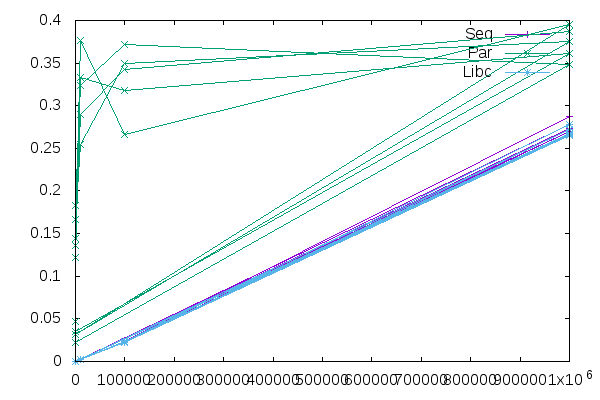
\includegraphics[width=.9\linewidth]{data/chevamax-Satellite-Pro-R50-B_2017-01-19/measurements_14:57_wide.png}

Oups\ldots{}

\begin{verbatim}
library("ggplot2")
df <- read.csv("data/chevamax-Satellite-Pro-R50-B_2017-01-19/measurements_14:57_wide.csv",header=T);
ggplot()+ geom_point(data=df, aes(x=Size, y=Seq, color="green"))+
  geom_point(data=df, aes(x=Size, y=Par, color="red")) + 
  geom_point(data=df, aes(x=Size, y=Libc));
\end{verbatim}

Petit test en R, mais je ne maitrise pas du tout ggplot \ldots{} Du coup
difficile d'analyser.

\section{Test 3}
\label{sec:orgheadline13}
Dans ce troisieme test nous allons affiner la courbe en faisant des tests
sur des tableaux de taille 10, 50, 100, 500, 1000, 5000, 10000, 50000,
100000, 500000 et 1000000.

Nous allons effectuer le test 10 fois pour chaque valeur.


\begin{verbatim}
scripts/run_benchmarking.sh
\end{verbatim}
\begin{verbatim}
OUTPUT_DIRECTORY=data/`hostname`_`date +%F`
mkdir -p $OUTPUT_DIRECTORY
OUTPUT_FILE=$OUTPUT_DIRECTORY/measurements_`date +%R`.txt

touch $OUTPUT_FILE
for i in 10 50 100 500 1000 5000 10000 50000 100000 500000 1000000; do
    for rep in `seq 1 10`; do
        echo "Siz
\end{verbatim}



Pour trasformer le fichier texte en fichier on utilise le script
fourni et la commande :

\begin{verbatim}
FILENAME="data/chevamax-Satellite-Pro-R50-B_2017-01-19/measurements_16:12"
perl scripts/csv_quicksort_extractor2.pl < "$FILENAME.txt" > "${FILENAME}_wide.csv"
\end{verbatim}

\begin{verbatim}
library("ggplot2")
df <- read.csv("data/chevamax-Satellite-Pro-R50-B_2017-01-19/measurements_16:12_wide.csv",header=T);
ggplot()+ geom_point(data=df, aes(x=Size, y=Seq, color="green"))+
  geom_point(data=df, aes(x=Size, y=Par, color="red")) + 
  geom_point(data=df, aes(x=Size, y=Libc));
\end{verbatim}


\subsection{Compilons en -O3}
\label{sec:orgheadline12}

\begin{verbatim}
FILENAME="data/chevamax-Satellite-Pro-R50-B_2017-01-19/measurements_16:24"
perl scripts/csv_quicksort_extractor2.pl < "$FILENAME.txt" > "${FILENAME}_wide.csv"
\end{verbatim}

\begin{verbatim}
library("ggplot2")
df <- read.csv("data/chevamax-Satellite-Pro-R50-B_2017-01-19/measurements_16:12_wide.csv",header=T);
ggplot()+ geom_point(data=df, aes(x=Size, y=Seq, color="green"))+
  geom_point(data=df, aes(x=Size, y=Par, color="red")) + 
  geom_point(data=df, aes(x=Size, y=Libc));
\end{verbatim}
\end{document}